Systems that need to perform multiple tasks face a fundamental trade-off problem: they cannot reach optimal performance in all tasks at once. Any such system, however, will have a set of solutions that are \textit{Pareto optimal} (also \textit{Pareto efficient}) for which a performance increase in one task must be traded for a performance decrease in another. Informally, trade-off situations that motivate Pareto optimal decision making are common in everyday desicion making; e.g. when a consumer, strictly concerned with cost and comfort, is looking to buy a car, her set of favorite candidate models will form the Pareto front, i.e. cars that minimize cost and maximize comfort. Pareto optimal states - of which there may be infinitely many for a system - form a set in performance-space called the \textit{Pareto front}. States that are not on the Pareto front are not Pareto optimal because there exists states which has higher performance of one task without compromise. Fig. \ref{fig:paretoOptimality} illustrates this concept.

\begin{figure}[h]
\centering
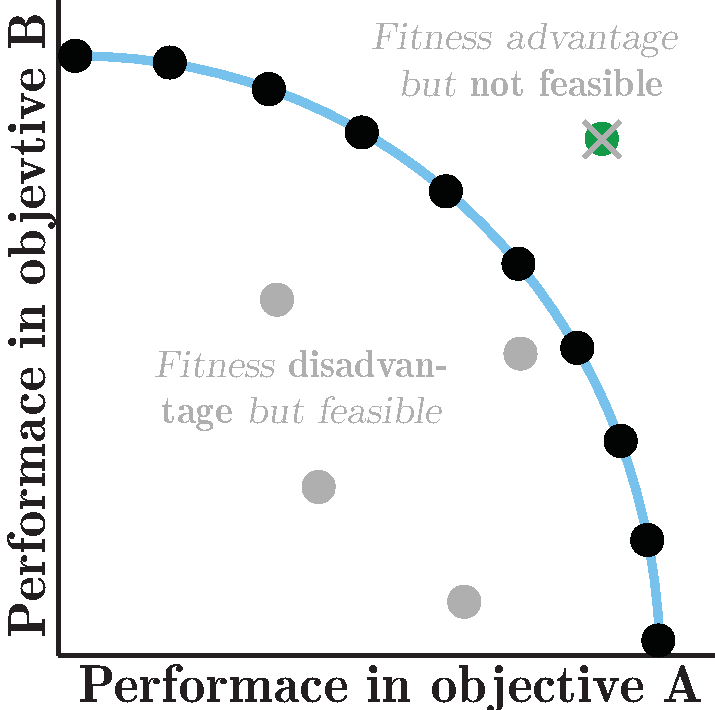
\includegraphics[width=0.5\linewidth]{figures/paretoOptimality.pdf} 
\caption{Example of a Pareto front for a two-task system. The set of states along the blue line form the Pareto front because niether can be optimized in one task without compromising performance in the other. Gray points illustrate states that not Pareto optimal, because there exists states that do increase performance in one task without compromise.}
\label{fig:paretoOptimality}
\end{figure}

The concept of Pareto optimality mainly finds applications in engineering, economics and logistics, dealing with as resource allocation, risk taking in investment banking, load distribution in electrical energy systems and many other multi-objective optimization problems. Recent efforts in Systems Biology has furthermore proved the concept useful for explaining evolution of gene expressions in cells and phenotypes on various species\mcite{firstthing, secondthing}.